% !TeX spellcheck = de_DE

\section{Code Architektur}

In diesem Kapitel wird der Architektonische Aufbau des Projekts, sowie prägnante Schlüssel Codestellen, die unter anderem als Meilensteine zur Lösung des Ausgangsproblems darstellen. Der Grundsätzliche Aufbau kann der nachfolgenden Abbildung \ref{fig:OV} entnommen werden.

\begin{figure}[hbt!]
	\centering      
	\def\svgscale{0.75}
	\includesvg[inkscapelatex=false]{figures/OV.svg}
	\caption{Projektüberblick}
	\label{fig:OV}
\end{figure}

Das StreamWriter Modul kommuniziert mit jeweils dem C++ CUDA bzw. dem Python CUDA Modul mithilfe des TCP-Protokolls. Diese Verarbeiten die darüber empfangenen Daten und senden diese über eine weitere TCP-Verbindung zu einem Modul \texttt{Bokeh Server}. Dies ist ein Webserver mit vorgefertigten Techniken zur visuellen Aufbereitung von Daten. Die Empfangenen Daten werden per AJAX-POST Anfrage an den Browser weitergeleitet und mit Javascript zur Laufzeit visualisiert. Die Module beschreiben jeweils eigenständige Programme, die über TCP-Verbindungen kommunizieren. Der generelle Ablauf geschieht nach Abbildung \ref{fig:OV} von links, nach rechts. Im Projektverzeichnis befindet sich ein Batch-Skript zur Automatisierung dieses Ablaufs, das den Startvorgang der einzelnen Module in der gewünschten Reihenfolge gewährleistet und für einen Reibungslosen Ablauf sorgt. Zunächst wird das Modul StreamWriter gestartet. Danach wird dem Benutzer die Entscheidung über die CUDA-Variante durch eine Benutzereingabe überlassen. Das Python- bzw. C++ Modul startet durch die Eingabe '1' bzw. '2'. Eingehende TCP-Pakete des StreamWriters beschreiben die Audiodaten und werden je nach ausgewähltem Modul bzw. Sprache anders Verarbeitet. Die Ausgabe an den Bokeh Server liegt jedoch bei beiden Modulen in gleich Form vor. Aus den eingehenden periodischen Signalen entstehen somit über die Verschiedenen Verarbeitungsschritte und parallele Abläufe klar visualisierte harmonische Frequenzwert Anteile einer Audiodatei. 

Im folgenden werden nähere Einzelheiten der einzelnen Module thematisiert.

\subsection{StreamWriter}
\label{sub:StreamWriter}

Das Teilprojekt \texttt{StreamWriter} dient als Schnittstelle zur Aufbereitung der Audiodaten aus den WAV-Dateien, Sammlung dieser Daten bis zu einem bestimmten Schwellwert und anschließender Weiterleitung über eine TCP Verbindung zum C++ bzw. Python CUDA Modul. Die Main Routine implementiert ein \texttt{fileConfig} Objekt, in dem die wichtigsten Angaben gebündelt werden. Die Variable \texttt{format} kann die beiden Werte DataFormat::WAV und DataFormat::RAW annehmen. Erstere Angabe dient interpretiert die Eingabedatei als vollwertige WAV-Datei. Dabei müssen die in Kapitel \ref{sub:WAV} beschriebenen Headerinformationen ausgewertet werden. DataFormat::RAW betrachtet die Datei als Rohformat. Hierfür müssen jedoch wichtige Angaben, die normalerweise im Header gespeichert sind, angegeben werden. Die wichtigsten Angaben sind:
\begin{itemize}
	\item Anzahl der Audiokanäle (int channels)
	\item Größe der einzelnen Samples in Byte (int BytesPerSample)
	\item Sample Rate (int sampleRate)
	\item Schwellwert der gleichzeitig verarbeiteten Audiosamples (int threshhold)
\end{itemize}

Außerdem wird hier der Pfad zur Eingabedatei in der Variablen std::string inFile spezifiziert.
Beide Fälle der Eingabeformate durchlaufen eine ähnliche Routine und werden mithilfe eines Switch-Case Konstrukts differenziert. Der gravierende unterschied zwischen beiden ist, dass für das Format DataFormat::RAW keine Headerinformationen zur Verfügung stehen und somit nicht aus der Datei extrahiert werden müssen. Daher liegt der Fokus im Folgenden auf dem Fall einer Angabe des Formats DataFormat::WAV.

\begin{figure}[t!]
	\lstinputlisting[frame=none, language=C, firstline=17, lastline=25, firstnumber=17 ]{../../Master\_parallel\_fourier\_audio/StreamWriter/Writer.h}
	\caption{fileConfig struct}
	\label{fig:fileConfig}
\end{figure}

Der DataFormat::WAV Fall des Switch-Case ist in Abbildung \ref{fig:WriterCPP} demonstriert. Der Ablauf beginnt in Zeile 57 mit der Erstellung eines WAVLoader Pointers mit \texttt{WAVLoader* = new\_WAVLoader((char*)file\_in.c\_str());}. An dieser Stelle wird die Eingabedatei dem WAVLoader Objekt übergeben, welches Headerinformationen und die eigentlichen Audiodaten extrahiert und in einem - abhängig von der Anzahl der Audiokanäle - zweidimensionalen Array gespeichert. Ein Meilenstein bei der Erstellung des WAVLoader Objekts war die Erkenntnis, dass das Lesen von Dateien, welche im Binärformat vorliegen, auch im Binärmodus geöffnet werden müssen. Die Funktion \texttt{fopen\_s} akzeptiert als dritten Parameter diese Art von Zugriffsmodi. Die Angabe von \texttt{'rb'} garantiert dabei lesenden Zugriff auf die Datei im Binärmodus. Während dies bei herkömmlichen Textdateien irrelevant ist, werden durch die Nichtangabe des Schalters \enquote{b} Wagenrückläufer \enquote{\textbackslash n} und Zeilenvorschübe \enquote{\textbackslash r} übersetzt. 

\begin{figure}[t!]
	\lstinputlisting[frame=none, language=C, firstline=22, lastline=26, firstnumber=22 ]{../../Master\_parallel\_fourier\_audio/StreamWriter/WAV.c}
	\caption{Eingabe Datei im Binärmodus lesen}
	\label{fig:openFile}
\end{figure}

Dies würde bei WAV-Dateien dazu führen, dass die Hexadezimalwerte z.B. \enquote{0x0A - 10} und \enquote{0x0D - 13} als Steuerzeichen interpretiert werden, sodass falsche Eingabewerte übersetzt würden. In Grafik \ref{fig:differenceGraph} ist zu erkennen, wie schnell kleine Fehler zu falschen Ergebnissen führen können. Aus diesem Grund wird hier die Gegenüberstellung zwischen dem falschen (oben) und dem richtigen (unten) Eingabesignal präsentiert.

\begin{figure}[hbt!]
	\centering      
	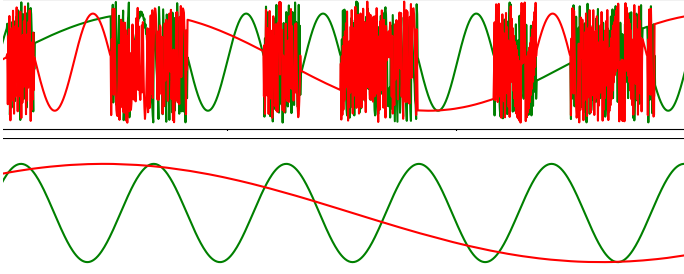
\includegraphics[scale=0.5]{figures/layerDifference.png}
	\caption{Vergleich fopen\_s mit Modi \enquote{r} (oben) und \enquote{rb} (unten)}
	\label{fig:differenceGraph}
\end{figure}

Der untere Graph zeigt auch unter anderem die erstellte Testdatei, in der zwei harmonische Sinuswellen (300hz und 40hz) auf auf jeweils dem linken bzw. rechten Audiokanal überlagert sind.

Im weiteren Verlauf der Instanziierung des WAVLoader Objekts werden hauptsächlich Daten der Ausgangsdatei mithilfe der Funktion \texttt{fread()} ausgelesen und in Membervariablen gespeichert. Das zuvor genannte zweidimensionale Array, welches die Sampledaten speichert, wird wie folgt realisiert:

\newpage
\begin{lstlisting}[language=C, frame=none]
	int **channelArr = (int**) malloc(sizeof(int*) * self->fmt.NumChannels);
	// allocate memory for all samples for each channel
	for (int i = 0; i < self->fmt.NumChannels; i++)
	channelArr[i] = (int *)malloc(sizeof(int) * (self->data.SampleNumber) + 1);
\end{lstlisting} 

Die Daten der Kanäle werden auf int Pointer abgebildet, die wiederum von int Pointern Referenziert sind, deren Größe mit der Anzahl der Samples bzw. Anzahl der Kanäle skaliert ist. Je nach Eingabegrößen muss der entsprechende Speicherplatz hier angepasst werden.

Abbildung \ref{fig:extractionSamples} zeigt die Speicherung der Daten in diesen beschriebenen Arrays. Anzumerken ist, dass die einzelnen Samples in einen Buffer der entsprechenden Größe eines Samples gelesen wird. Möglicherweise muss für die anschließende Zuweisung im Pointer eine Anpassung der Bytereihenfolge (Endianness) stattfinden. Dazu wird der Inhalt des Buffers durch \texttt{memcpy(\&num, buffer, 4);} in einen 4 Byte Integer umgewandelt und in der entsprechenden Bytereihenfolge gespeichert.

\begin{figure}[t!]
	\lstinputlisting[frame=none, language=C, firstline=91, lastline=116, firstnumber=91 ]{../../Master\_parallel\_fourier\_audio/StreamWriter/WAV.c}
	\caption{Hauptiteration: Extraktion der Sample Daten}
	\label{fig:extractionSamples}
\end{figure}

Die Sample Daten der WAV-Datei sind an dieser Stelle geladen und durch Pointer im WAVLoader Objekt zugänglich. Der nächste Schritt in Zeile 58 \ref{fig:WriterCPP} ist eines \texttt{Sender()} Objekts. Der Konstruktor ruft die Member Methode texttt{Initlialize(std::string host, std::string port)} auf, die einen Socket auf localhost mit dem Port 1337 bindet und auf eingehende Verbindungen wartet. Dafür wurde die Windows API verwendet, demnach ist das Programm nur auf dieser Plattform lauffähig. Für die Kombatibilität mit Linux Distributionen müssten an dieser Stelle Änderungen implementiert werden. Die implementierte Funktion \texttt{int Sender::Send(std::string msg)} sendet den angegebenen String über den TCP-Socket an die entsprechenden angedockten Endpunkte. 


\begin{figure}[t!]
	\lstinputlisting[frame=none, language=C, firstline=54, lastline=92, firstnumber=54 ]{../../Master\_parallel\_fourier\_audio/StreamWriter/Writer.cpp}
	\caption{StreamWriter Main Loop}
	\label{fig:WriterCPP}
\end{figure}

Die Zeilen 62 bis 86 implementieren eine Schleifenoperation, in der die zuvor gespeicherten Sample Daten in einem \texttt{stringstream} zusammengesetzt werden. Die Samples sind in Hexadezimalform im String gespeichert. Der Vorteil liegt darin, dass sich die Anzahl der Zeichen für die repräsentierten Dezimalzahlen nicht vergrößert. Die Samplegröße bestimmt die Bytegröße und somit die Länge der Hexadezimal Strings. Um eine gleichbleibende String-Struktur beizubehalten, werden die Hexwerte wenn nötig auf die passende Länge erweitert und mit voranstehenden Nullen aufgefüllt.

\begin{lstlisting}[language=C, frame=none]
	ss << std::setfill('0') << std::setw(4) << std::hex << static_cast<uint32_t>(sample);
\end{lstlisting} 

Anschließend wird der mit dem \texttt{stringstream} Objekt konstruierte String mit der Funktion Send() des Sender Objekts über die TCP-Schnittstelle verfügbar gemacht.

An dieser Stelle ist die Aufgabe des StreamWriter Moduls abgeschlossen. Die präsentierte Endlosschleife wird so lange durchgeführt, bis alle Sampledaten des WAVLoader Objekts erfolgreich auf der Gegenseite empfangen wurden. Zuletzt erfolgen diverse Aufräumarbeiten bzw. Memory Cleanup.

\begin{lstlisting}[language=C, frame=none]
	sender->Send(ss.str());
\end{lstlisting}

\paragraph{Datei-Variante}
	- evtl. aufteilen
\paragraph{TCP-Variante}
	- evtl. aufteilen
	
\subsection{AudioTracer} \label{sec:audiotracer}

Die nächsten zwei Sektionen umschließen den Hauptteil des Programmatischen Teils dieser Arbeit. Die Implementierung der Module AudioTracer in C- und Python- Variante. Die beiden Module erfüllen dieselbe Aufgabe, arbeiten jedoch unabhängig voneinander und werden nicht parallel ausgeführt. Die zu verarbeitenden Daten werden vom StreamWriter Modul über bereits angesprochene TCP-Schnittstellen empfangen. Dafür werden analog zum StreamWriter Modul Socket Implementierungen vorgenommen, die die Audio Samples empfangen. Die Sockets knüpfen dabei aktiv an die horchende Gegenseite des StreamWriters an. Als Vorgriff ist anzumerken, dass hier bereits die Verbindung zum Bokeh-Visualisierungsmodul initialisiert wird. Dieser Teil wird später in Sektion \nameref{sec:bokeh} thematisiert. Im Folgenden unterscheiden sich die Implementierungen der AudioTracer Module und werden daher getrennt genauer beschrieben.

\paragraph{AudioTracer (C)}

Die C Version des AudioTracers implementiert die Methode initSocket(). Aufgabe dieser Methode ist es, eine Verbindung zu einer Host Adresse mit gegebenem Port herzustellen und aufrecht zu erhalten. Der Grundsätzliche Ablauf zur Erstellung und Verbindung eines Sockets mit der entsprechenden Gegenstelle ist in der Windows API folgendermaßen zu erreichen:

\begin{lstlisting}[language=C, frame=none]
	bool initSocket(SOCKET& s, char* host, int port)
	{
		struct sockaddr_in server;
		WSADATA wsa;
		WSAStartup(MAKEWORD(2, 2), &wsa);
		s = socket(AF_INET, SOCK_STREAM, 0);
		server.sin_addr.s_addr = inet_addr(host);
		server.sin_family = AF_INET;
		server.sin_port = htons(port);
		connect(s, (struct sockaddr*)&server, sizeof(server));
		return true;
	}
\end{lstlisting}

Die Ausgaben und Statusabfragen auf Konsistenz der erzeugten Objekte bzw. Rückgabewerte der Methoden werden in diesem Codestück zu Vereinfachung nicht aufgeführt, sind aber in Abbildung \ref{fig:initSocket} vollständig aufgelistet. Im struct socketaddr\_in werden alle Informationen der Verbindung festgehalten, welche in den Zeilen 7 bis 9 festgelegt werden. Die Host Adresse liegt als Char Pointer vor und muss mithilfe der Funktion inet\_addr(char*) in den Typ in\_addr umgewandelt werden (Zeile 7). Selbiges gilt für die Portnummer, welche als int vorliegt und in den Typ USHORT mit htons() umgewandelt wird (Zeile 9). Die Variable sin\_family hat den Typ ADDRESS\_FAMILY und kann die Werte AF\_UNSPEC, AF\_INET und AF\_INET6 annehmen. Hier wird der Wert AF\_INET verwendet. Dadurch wird die Verbindung über das IPv4 Protokoll aufgebaut. AF\_INET6 wäre für eine IPv6 Verbindung anzugeben.
Die Winsock DLL wird über die Funktion:
\begin{lstlisting}[language=C, frame=none]
	int WSAStartup(
	WORD      wVersionRequired,
	LPWSADATA lpWSAData
);
\end{lstlisting}

MAKEWORD(2, 2) in Zeile 5 gibt dabei die zu verwendende Version der Winsock DLL an. In diesem Fall wird Version 2.2 vorausgesetzt. Der Socket wird in Zeile 6 konstruiert. Die Methode socket akzeptiert als ersten Parameter die verwendete ADDRESS\_FAMILY. Auch hier wird AF\_INET und somit IPv4 verwendet. Der zweite Parameter gibt den Typ des Sockets an. Für den Verwendungszweck ist nur der Wert  SOCK\_STREAM sinnvoll. Die offizielle Dokumentation \cite{ms_docs_winsock} gibt dazu folgende Beschreibung her:\enquote{A socket type that provides sequenced, reliable, two-way, connection-based byte streams with an OOB data transmission mechanism. This socket type uses the Transmission Control Protocol (TCP) for the Internet address family (AF\_INET or AF\_INET6).} TCP ist offensichtlich sinnvoll, um die erfolgreiche Übertragung der Daten zu gewährleisten. Der dritte Parameter ist das Protokoll des Sockets selbst. Durch die Angabe des Wertes 0 wird dieses vom Service Provider, in diesem Fall StreamWriter Socket, festgelegt.

\begin{lstlisting}[language=C, frame=none]
	SOCKET WSAAPI socket(
	int af,
	int type,
	int protocol
	);
\end{lstlisting}

Zuletzt wird die Verbindung durch den Aufruf der folgenden Methode aufgebaut:
\begin{lstlisting}[language=C, frame=none]
	int WSAAPI connect(SOCKET s, const sockaddr *name, int namelen);
\end{lstlisting}

An diesem Punkt akzeptiert der StreamWriter Socket die Verbindung und startet somit den in Sektion \nameref{sub:StreamWriter} beschriebenen Ablauf. Die nächsten Schritte der Main Methode des AudioTracer(C)-Moduls implementieren eine Schleifenoperation, die für das Empfangen, sowie die eigentliche Verarbeitung der Daten zuständig ist. Zunächst müssen dafür jedoch einige Vorbereitungen getroffen werden. Analog zum StreamWriter Modul werden die Sampledaten in einem Array gespeichert. Dieses wird im Voraus mit entsprechendem Speicherplatz bis zu einem Schwellwert (THRESHHOLD) initialisiert. Die Zeilen 1 bis 3 realisieren diesen Schritt in folgendem Codeschnipsel.

\begin{lstlisting}[language=C, frame=none]
	int** sampleData = (int**)malloc(sizeof(int*) * channelNumber);
	for (int i = 0; i < channelNumber; i++)
		sampleData[i] = (int*)malloc(sizeof(int) * THRESHHOLD);
	
	int arr_pos = 0;
	long start = 0;
	int rcvSize = (channelNumber * sampleSize + channelNumber - 1 + 1) * THRESHHOLD;
	char* rcvBuf = (char*)malloc(sizeof(char) * channelNumber * THRESHHOLD);
	char* startptr, *endptr;
\end{lstlisting}

Außerdem werden für die darauffolgende Schleifenoperation wichtige Variablen angelegt, die zur Positionsbestimmung (Z. 5f.) und Extraktion der Daten aus dem TCP-Stream (Z. 8f.) zuständig sind. Der innere Ablauf der while(true) Anweisung lässt sich in zwei Bereiche aufteilen. Der hintere Teil der Schleife ist in Abbildung \ref{fig:whileFirst} demonstriert. Die Zeilen 312 bis 316 implementieren das Empfangen der Daten, die zuvor vom StreamWriter Modul über die TCP-Schnittstelle gesendet wurden. Da im Regelfall ein kontinuierlicher Datenstrom beim Empfangen der Daten erwartet wird, werden so lange Daten von der Gegenseite angenommen, bis ein vom Schwellwert abhängiger Byte Wert empfangen wurde. Die Variable rcvSize gibt die zu erwartende Bytegröße nach der Formel im obigen Codefragment (Z. 7) an. Für jede Sample Gruppe wird die Anzahl der Kanäle mit der Samplegröße multipliziert. Die Kanäle werden mithilfe von Leerzeichen getrennt und von neuen Samplegruppen durch Newline Steuerzeichen getrennt. Multipliziert mit der maximalen Anzahl der gleichzeitig verarbeiteten Samplesgruppen ergibt dies die zu erwartende Größe der Daten, die über den TCP Stream empfangen werden , in Bytes an. Bei einem Schwellwert von 5000 Samples á vier Byte auf zwei Kanälen würden 50000
Bytes empfangen werden.

\begin{figure}[t!]
	\lstinputlisting[frame=none, language=C, firstline=301, lastline=326, firstnumber=301 ]{../../Master\_parallel\_fourier\_audio/Master\_parallel\_fourier\_audio/kernel.cu}
	\caption{Schleifenoperation: Hinterer Teil}
	\label{fig:whileFirst}
\end{figure}

%todo eigentlich sind das 2 byte aber wegen string konvertierung 4 pro sample
Der Bereich von Zeile 321 bis 338 realisiert ein String Tokenizer, um aus dem empfangenen String die eigentlichen Daten zu extrahieren. Dabei werden wieder einzelne Samplegruppen mit einem Newline Steuerzeichen und einzelne Kanaldaten mit einem Leerzeichen separiert und mit der Methode strtol in Integer Werte konvertiert.
Dafür zeigen zunächst zwei Pointer (startptr und endptr) auf den Anfang des empfangenen Charpointers rcvBuf. Danach wird das Newline Steuerzeichen lokalisiert und der Pointer endprt auf dessen Position ausgerichtet. Die Zeichen des Strings zwischen endptr und startptr werden darauf folgend in einem neu erzeugten String Objekt \texttt{char* perChannel} kopiert. Die Variable perChannel enthält nun wiederum die Stringrepräsentierung einer Samplegruppe, die mithilfe von strtok() in einzelne Kanaldaten aufgespalten und somit in Integer umgewandelt in das Array sampleData kopiert werden können. Letztlich wird der Pointer startptr auf die Position von endptr + 1 gesetzt, um von dort aus das nächste auftreten eines Newline Steuerzeichens zu finden. Diese Vorgehensweise ist unter anderem ein Beispiel für einen nicht destruktiven String Tokenizer in C. Eine Variable arr\_pos zählt die bereits übertragenden Samplegruppen. Sobald diese den Schwellwert THRESHHOLD übersteigt, wird der Teil des Programms erreicht, der eine hohe Relevanz in dieser Arbeit einnimmt. Die Implementierung der Parallelisierung einer Fouriertransformation auf den bis jetzt übermittelten und extrahierten Daten über die CUDA Schnittstelle für Nvidia Grafikkarten.

\begin{figure}[t!]
	\lstinputlisting[frame=none, language=C, firstline=271, lastline=296, firstnumber=271 ]{../../Master\_parallel\_fourier\_audio/Master\_parallel\_fourier\_audio/kernel.cu}
	\caption{Schleifenoperation: Vorderer Teil}
	\label{fig:whileSecond}
\end{figure}

Die Implementierung der parallelisierten Fouriertransformation gibt die folgende Methodensignatur vor:
\begin{lstlisting}[language=C, frame=none]
	cudaError_t cudaFourierTransform(cplx* x, cplx* complexOut, int channelNb, int size)
\end{lstlisting}
Die Parameter x und complexOut werden als Pointer vom Typ cplx erwartet. Dieser Typ ist eine Abstraktion der CUDA-eigenen Bibliothek für komplexe Zahlen in float-Genauigkeit. Die Bereits empfangenen Daten liegen jedoch im Typ Integer vor. Aus Typkonsistenz Gründen müssen diese zum Typ cplx konvertiert werden. Außerdem ist die Arbeit mit mehrdimensionalen Arrays - bzw. in diesem Fall Pointer-auf-Pointer Konstrukten - schwierig, sodass hier zusätzlich eine Modulation in ein eindimensionales Array der Daten durchgeführt wird. Die cuComplex Bibliothek stellt die Methode make\_cuComplex zur Verfügung. Die Angabe von Real- und Imaginärteil einer Komplexen Zahl wird dafür erwartet. Da die Ausgangsdaten im Integer Format vorliegen und somit keinen Imaginärteil besitzen, wird dieser mit 0 angegeben. Zeilen 279 bis 286 in Abbildung \ref{fig:whileSecond} realisieren diese beiden Schritte.

Die Ausgabe der Fouriertransformation erfolgt in einem neu angelegten Pointer vom Typ cplx mit entsprechend allozierten Speicherplatz, abhängig zur Anzahl der Audiokanäle und THRESHHOLD (Z. 276). Aufgrund des Stellenwerts, den die Methode cudaFourierTranform einnimmt, wird diese in der hierauf folgenden Sektion separat beschrieben. Wichtig für den hier thematisierten Teil der AudioTracer Implementierung ist, dass der Pointer complexOut auf die Fouriertransformierten Rückgabewerte zeigt. In der Topologie der Implementierung nach Abbildung \ref{fig:OV} ist die Beschreibung mit der Methode sendBuf in Zeile 289 am Kantenübergang zwischen dem Modul AudioTracer(C) und Bokeh Server angelangt. Die Daten werden über den anfangs erstellten Socket s\_vis an den Server gesendet. Die grundsätzliche Vorgehensweise die Übermittlung der Daten in Form eines JSON Strings. Da es sich bei dem Bokeh Modul um einen Webserver handelt, ist eine solche Übertragung in gegenwärtiger JavaScript Umgebung sehr sinnvoll. Die Daten müssen lediglich in die Form eines JSON-Arrays gebracht werden. Der nötige Schritt ist die Umschließung der Kommaseparierten Daten mit \enquote{[} bzw. \enquote{]} und wird durch eine einfache Iteration in Verbindung mit der Funktion snprintf realisiert. Problematisch ist jedoch, dass die durch die Fouriertransformation entstandenen Ausgabedaten weiterhin im Format cplx* vorliegen. Komplexe Zahlen werden üblicherweise im kartesischen Koordinatensystem mit Real- und Imaginärteil angegeben. Mithilfe der Polarform lässt sich der Betrag einer komplexen Zahl errechnen:
\begin{flushleft}
	\textbf{Definition \eqref{eq:6}}: Polarform von komplexen Zahlen
\end{flushleft}
\vspace{\baselineskip}
\begin{equation}
	\begin{gathered}
		\text{Sei z eine komplexe Zahl in der Form} z = a + b * i. \\
		\text{Dann ist der absolute Betrag r definiert als:} \\
				r = |z| = \sqrt{a^{2} + b^{2}}
	\end{gathered}\label{eq:6}
\end{equation}

In der Implementierung wird dafür die Bezeichnung ftMagnitude verwendet:

\begin{lstlisting}[language=C, frame=none]
	float ftMagnitude = sqrtf(
	  cuCrealf(complx[c * threshhold + samp]) 
	* cuCrealf(complx[c * threshhold + samp]) 
	+ cuCimagf(complx[c * threshhold + samp]) 
	* cuCimagf(complx[c * threshhold + samp]));
	mag[c * threshhold + samp] = ftMagnitude;
\end{lstlisting}

Die Variablen c und samp beschreiben im Kontext einer Iteration der Sampledaten den aktuell betrachteten Kanal bzw. Sample aus diesem Kanal. Die Libraryfunktionen cuCrealf und cuCimagf lesen den Real- bzw. Imaginärteil analog zur Definition a bzw. b der komplexen Zahl aus. Der zusammengesetzte String wird über den vorhandenen Socket an den Bokeh Server gesendet.

Der folgende Part liefert genauere Einblicke in die Implementierung der Initialisierung der CUDA Schnittstelle Speicherverwaltung, sowie die Aufteilung der parallelisierten Fouriertransformation auf CUDA-Kernels und letztlich die Implementierung der Fouriertransformation selbst.

\paragraph{Einzelheiten der CUDA Implementierung}
Die vorherigen Kapitel dieser Arbeit beschreiben einen großen Vorbereitungsaufwand, um eine ursprüngliche Audiodatei im WAV Format für eine Implementierung einer Fouriertransformation verfügbar zu machen. Dabei wird die Datei interpretiert und deren Daten extrahiert. Diese werden über eine TCP-Schnittstelle versendet und von der Gegenseite empfangen und in einem entsprechenden Format bereitgestellt und für den nächsten Schritt vorbereitet.

\begin{figure}[t!]
	\lstinputlisting[frame=none, language=C, firstline=337, lastline=344, firstnumber=337 ]{../../Master\_parallel\_fourier\_audio/Master\_parallel\_fourier\_audio/kernel.cu}
	\lstinputlisting[frame=none, language=C, firstline=346, lastline=349, firstnumber=346 ]{../../Master\_parallel\_fourier\_audio/Master\_parallel\_fourier\_audio/kernel.cu}
	\lstinputlisting[frame=none, language=C, firstline=351, lastline=359, firstnumber=351 ]{../../Master\_parallel\_fourier\_audio/Master\_parallel\_fourier\_audio/kernel.cu}
	\lstinputlisting[frame=none, language=C, firstline=361, lastline=362, firstnumber=361 ]{../../Master\_parallel\_fourier\_audio/Master\_parallel\_fourier\_audio/kernel.cu}
	\lstinputlisting[frame=none, language=C, firstline=370, lastline=376, firstnumber=370 ]{../../Master\_parallel\_fourier\_audio/Master\_parallel\_fourier\_audio/kernel.cu}
	\lstinputlisting[frame=none, language=C, firstline=378, lastline=383, firstnumber=378 ]{../../Master\_parallel\_fourier\_audio/Master\_parallel\_fourier\_audio/kernel.cu}
	\caption{CUDA Vorbereitungen}
	\label{fig:cudaFourierTransform}
\end{figure}

Abbildung \ref{fig:cudaFourierTransform} zeigt die wichtigsten Codestellen und Überlegungen für den Abschluss der Vorbereitungsarbeiten der parallelen Transformation. Die Voraussetzung ist CUDA-fähige Hardware und die entsprechende Entwicklungsumgebung mit mindestens eingebundenen Cuda Bilbiotheken cuda\_runtime.h und device\_launch\_parameters.h.
Zeile 340 initialisiert das CUDA-fähige Gerät durch den Aufruf der Methode cudaSetDevice(int device). Die Spezifikationen des Entwicklungssystems ist in Sektion \ref{sub:gtx1080} beschrieben. Für diesen Fall steht ein Gerät zur Verfügung, somit ist diese mit dem Parameter 0 zu referenzieren. Bei multi-GPU Systemen würde an dieser Stelle der gewünschte Index angegeben. Informationen über die installierten GPU-Geräte können mithilfe von cudaGetDevice(int device) abgefragt werden. Für den Fehlerfall der CUDA Funktionen steht der Rückgabetyp cudaError\_t bereit. 

Grundsätzlich kann die Device-Umgebung nicht direkt auf den Host Adressraum zugreifen. Dafür müssen die verwendeten Daten auf den Device Adressraum und Rückgabewerte von diesem wieder auf das Host-System übertragen werden. Die Variablen cplx* dev\_c und cplx* dev\_out werden für diese Zwecke in den Zeilen 347f. auf dem Speicherbereich der Grafikkarte alloziert (cudaMalloc). Der anzugebene Pointer zeigt nach Ausführung von cudaMalloc auf den allozierten Speicher auf der Device Umgebung. Der Speicher für die Ausgabe muss lediglich auf der Grafikkarte initialisiert werden. Die Sampledaten müssen allerdings mit cudaMemcpy auf das Gerät kopiert werden. Die Parameter sind ein Pointer auf den Speicherbereich der Grafikkarte und ein weiterer, in dem sich die Daten befinden, die übertragen werden sollen. Die Richtung des Kopiervorgang muss hier explizit angegeben werden. Die nötigen Angaben sind cudaMemcpyHostToDevice für das Kopieren in Device Richtung und cudaMemcpyDeviceToHost für die Rückrichtung.

Für die parallele Ausführung von CUDA Kernels, muss vorher ein entsprechendes Muster angelegt werden. Hierfür werden dreidimensionale Vektoren verwendet. Ab einer gewissen Größe der Eingabedaten, in diesem Anwendungsfall Anzahl der Audiosamples, wird ein Maximum an parallel ausführbaren Kernels erreicht. Aus diesem Grund können nicht alle Daten parallel verarbeitet werden. Die auszuführenden Threads sind in einem System von CUDA Grids und Blocks angegeben. Je nach Dimension dieser als Vektoren angegebenen Variablen ändert sich die Anzahl der Threads auf den CUDA Kernels. 

\begin{figure}[hbt!]
	\centering      
	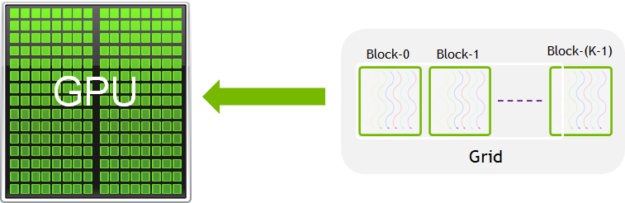
\includegraphics[scale=0.5]{figures/cudaGrid.png}
	\caption{Topologie der CUDA Kernels \cite{nvidia_docs_grid}}
	\label{fig:cudaGrids}
\end{figure}

In Abbildung \ref{fig:cudaGrids} ist die Topologie der GPU abgebildet. Ein CUDA Grid (links) besteht aus den rechts abgebildeten Blöcken (Block-0 ... Block-(K-1)). In jedem dieser Blöcke wird eine definierte Anzahl an Threads ausgeführt, die hier in Wellenförmigen Pfeilen dargetstellt werden. 

In Zeile 351 wird die maximale Anzahl der Threads in einem Block (1024) für die Entwicklungsumgebung verwendete GPU angegeben. Die weitere Berechnung der Grid- und Blockdimensionen basieren unter Anderem auf dieser Angabe. Die Überlegung zur Aufteilung, welche in den Zeilen 352 bis 356 durchgeführt wird, geht dahin, dass die Grid Dimensionen abhängig von der Anzahl der Audiokanäle sowie Anzahl der Samples wachsen.
Die Variable threadCluster in Zeile 352 berechnet sich durch die Divison der Eingangsgröße durch die maximale Anzahl der Threads in einem Block. Um Datenverlust zu verhindern, wird dieses Ergebnis auf den nächst größeren Integer Wert aufgerundet. Mithilfe der Variablen channelNumber und threadCluster können die Dimensionen des CUDA-Grids (Z. 358f) definiert werden. Dabei bestimmen threadCluster bzw. channelNumber die Größe in X- bzw. Y-Richtung. Die Länge der Z-Richtung des Vektors nimmt den Wert 1 an, da eine abweichende Angabe hier nicht notwendig ist. Die Größe der Blöcke im angegebenen Grid wird in Abhängigkeit der threatCluster berechnet und in der Variable actualThreadsPerBlock gespeichert (Z. 353 u. 356). Die Größe wird mit einer Division der Anzahl von Eingabesignalen durch die zuvor berechneten threadCluster definiert. Die Notwendigkeit von Mehrdimensionalen Blockvektoren wird hier nicht gesehen. Somit bestimmt die Variable actualThreadsPerBlock die Länge des Blockvektors in X-Richtung. Die Größen der Grid- und Blockdimensionen werden in Abbildung  \ref{fig:exampleGrid} visualisiert. Die Berechnung basiert auf folgenden Eingabegrößen:

\begin{itemize}
	\item maxThreadsPerBlock = 1024
	\item size = 5000
	\item channelNumber = 2
\end{itemize}

Mithilfe der Abbildung wird die allgemeine Struktur der Kernelausführung klarer.

\begin{figure}[hbt!]
	\centering      
	\def\svgscale{0.75}
	\includesvg[inkscapelatex=false]{figures/grid.svg}
	\caption{Gridbeispiel}
	\label{fig:exampleGrid}
\end{figure}

Jeder ausgeführte Thread hat Zugriff auf die Variablen blockIdx, blockDim, gridDim und threadIdx. Damit lässt sich zu jeder Zeit identifizieren, an welcher Stelle im Grid sich der aktuell betrachtete Thread befindet. Diese Information wird für den Zugriff auf die Pointer der Sampledaten verwendet. 

\begin{figure}[t!]
	\lstinputlisting[frame=none, language=C, firstline=129, lastline=133, firstnumber=129 ]{../../Master\_parallel\_fourier\_audio/Master\_parallel\_fourier\_audio/kernel.cu}
	\caption{CUDA Kernel}
	\label{fig:cudaKernel}
\end{figure}

In Listing \ref{fig:cudaKernel} ist die Implementierung der Kernelfunktion angegeben. In Zeile 135 ist zu erkennen, dass die Funktion als \_\_global\_\_ deklariert ist. Diese Direktive ermöglicht das Aufrufen von Funktionen im Speicherbereich des Device Systems. In diesem Fall ruft das Host System die Methode addKernel (Abbildung \ref{fig:cudaFourierTransform} Zeile 362) im Speicherbereich der Grafikkarte auf. Mithilfe des Operators \enquote{$<<<$ $>>>$} werden die zuvor berechneten Dimensionen von Grid und Blocks als Parameter überreicht. Analog dazu gibt es die Direktive \_\_device\_\_. Die so annotierten Funktionen können nur im Adressbereich der GPU referenziert werden und sind über das Host System nicht erreichbar. Die globale Funktion addKernel ruft die Methode \_dft auf, die das Herzstück der Kernelausführung bildet. Die Auflistung \ref{fig:devicedft} liefert die Implementierung einer diskreten Fouriertransformation, die in jeweils einem CUDA-Kernel durchlaufen wird. In den Zeilen 36 bis 39 werden die notwendigen Index-Informationen berechnet. Da jeder Kernel Zugriff auf den Ausgabe Pointer hat, muss die Referenzierung der Pointerpositionen eindeutig sein. Abbildung \ref{fig:exampleGrid} hilft dabei, diesen Vorgang zu veranschaulichen.
\begin{itemize}
	\item threadNumInBlock: Gibt den Index des Threads im aktuellen Block an und wird durch threadIdx.x + blockDim.x * threadIdx.y bestimmt. In der Skizze würde zum Beispiel Thread $t_{200}$ vom Block(0, 1, 1) angenommen. threadIdx.x wäre hier 200 und blockDim.x = 1000. Die Threads sind eindimensional angegeben, deshalb betragen y und z Werte von threadIdx jeweils 1.
	Somit ergibt sich ein Threadindex innerhalb des Blocks bei gegebenem Beispiel von $200 + 1000 * 0 = 200$
	\item side: Gibt den Index in Abhängigkeit des Blockindizes in Y-Richtung an. Analog zur Abbildung beschreibt dies den Anfangsindex einer Seite mit gleicher Y-Koordinate im Blockindex und ist mit $gridDim.x * blockIdx.y * blockDim.x$ angegeben. Beispielsweise wäre der Index zum Anfang der \enquote{rechten} Seite der Abbildung $5 * 1 * 1000 = 5000$
	\item sideIndex: Der Index innerhalb einer hier so genannten Seite lässt sich durch $blockIdx.x * blockDim.x + threadNumInBlock$. Für den im ersten Punkt genannten Thread lautet der Index $0 * 1000 + 200 = 200$.
	\item globalIndex: Gibt den globalen Index des Threads im Gridsystem an. Beide dafür notwendigen Parameter side und sideIndex sind dafür bereits gegeben und werden addiert:
	$5000 + 200 = 5200$
\end{itemize}

Die Variablen sideIndex und globalIndex werden für die Berechnung der Fouriertransformation sowie für die Positionsbestimmung im Ausgabearray verwendet.
In \eqref{eq:2} wurde bereits die Definition der diskreten Fouriertransformation vorgestellt. Mithilfe von \eqref{eq:3} wird klar, dass der Exponent $e^{\frac{-ikl\cdot 2\pi}{N}}$ in Real- und Imaginärteil umgewandelt werden kann: $\cos(\frac{2\pi}{N}kl) - i \cdot \sin(\frac{2\pi}{N}kl)$. Die passt in sofern auf die Implementierung, dass die Exponent im Typ cplx vorliegen muss, die weiteren Rechenschritte ausführen zu können. Zeile 44 führt diesen Schritt aus, wobei die eben genannten Indizes sideIndex und globalIndex verwendet werden. Nach der Formel wird dieser Exponent mit Audiosample multipliziert und das Ergebnis zur Ausgabe aufsummiert. Analog wird in Zeile 45 cuCmulf bzw. cuCaddf verwendet. Der Dämpfungsfaktor $1/N$ wird in der Implementierung nicht verrechnet, da dieser keine Auswirkung auf die zu observierenden Ergebnisse hat.

Das Hostsystem wartet durch den Methodenaufruf cudaDeviceSynchronize() im Programmablauf auf die Beendigung aller erstellten Threads. Sind diese erfolgreich zum Abschluss gekommen, muss das Ausgabearray dev\_out im Speicherbereich der GPU wieder in das Host System kopiert werden. Dies wird realisiert durch einen erneuten Aufruf von cudaMemcpy mit der Richtungsangabe cudaMemcpyDeviceToHost.

Hier angekommen wurde ein erfolgreicher Durchlauf einer parallel ausgeführten Fouriertransformation beschrieben. Der Host Programmablauf wartet nun auf Pakete, die zur TCP-Schnittstelle gesendet werden, um die Iteration mit neuen Daten erneut zu durchlaufen.

\begin{figure}[t!]
	\lstinputlisting[frame=none, language=C, firstline=32, lastline=48, firstnumber=32 ]{../../Master\_parallel\_fourier\_audio/Master\_parallel\_fourier\_audio/kernel.cu}
	\caption{Kernelfunktion \_dft}
	\label{fig:devicedft}
\end{figure}

\begin{figure}[hbt!]
	\centering      
	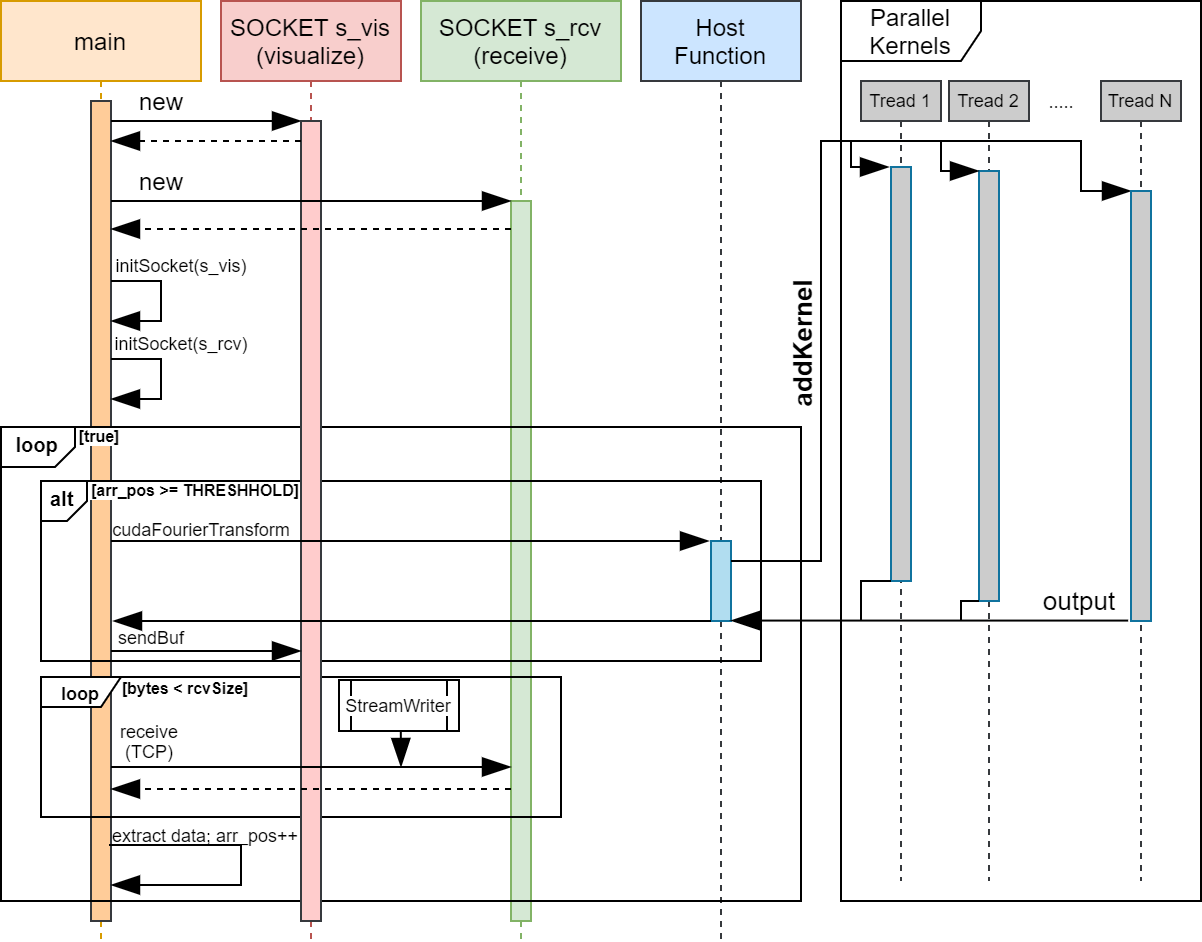
\includegraphics[scale=0.46, angle=-90]{figures/AudioTracerC++_sequence_diagram.png}
	\caption{Sequenzdiagramm AudioTracer-C}
	\label{fig:Seq_AudioTracer}
\end{figure}


\paragraph{AudioTracer (Python)}
Die Python Version des AudioTracer Projekts weist generell die gleiche Semantik wie das C Modul auf, hat jedoch einige Besonderheiten. Vor allem fällt die Kompaktheit des Python Moduls direkt auf. In ca. 100 Zeilen Code werden Daten empfangen, verarbeitet (fouriertransformiert) und zum Bokeh Modul weiter versendet. Dies liegt unter anderem an vielen hilfreichen Operatoren und vorgefertigten Methoden, die ein künstliches aufblähen des Codes verhindern. So wird z.B. in zwei Zeilen Code (Abbildung \ref{fig:pySocket}) ein voll funktionsfähiges Socket Objekt erstellt, über das Daten gesendet bzw. empfangen werden können. 

\begin{figure}[t!]
	\lstinputlisting[frame=none, language=C, firstline=47, lastline=49, firstnumber=47 ]{../../Master\_parallel\_fourier\_audio/python/pyCudaAudioTracer.py}
	\caption{Erstellung eines Sockets in Python}
	\label{fig:pySocket}
\end{figure}

Beim Umgang mit den Empfangenen Daten des StreamWriter Moduls ersetzt die Funktion split() aufwändige Pointer-Arithmetik, wie sie im C-Modul verwendet wurde. Auch die Konvertierung der Hex-Strings wird in einem Einzeiler durchgeführt:
\begin{lstlisting}[language=Python, frame=none]
	sample = int(perChannel[c], 16)
\end{lstlisting}
Gegebenenfalls müssen hier die verwendeten Bits bei größeren Datentypen der Eingangssignale angepasst werden. Auch das Senden der Fouriertransformierten Daten über den Socket des Bokeh Server funktioniert mit geringerem Aufwand:

\begin{lstlisting}[language=Python, frame=none]
json_str = json.dumps(freq_magnitudes)
send_data(visSocket, (str(len(json_str))+'|').encode('utf-8'))
send_data(visSocket, json_str.encode('utf-8'))
\end{lstlisting}

Die bereitgestellte Methode dumps des json Packages ermöglicht es das Array der Ausgabedaten in einen JSON-String zu konvertieren. Dieses kann ohne weiter Stringmanipulationen über den Socket des Bokeh Webservers gesendet bzw. empfangen werden.
Folgende Abbildung \ref{fig:fftpy} zeigt eine Implementierung der Fast Fourier Transformation (FFT) !!subject to change!! mithilfe der cupy-Library und anschließende Umwandlung der komplexen Ausgabedaten in deren absoluten Beträge.

\begin{figure}[t!]
	\lstinputlisting[frame=none, language=C, firstline=53, lastline=61, firstnumber=53 ]{../../Master\_parallel\_fourier\_audio/python/pyCudaAudioTracer.py}
	\caption{Erstellung eines Sockets in Python}
	\label{fig:fftpy}
\end{figure}

In Zeile 53 wird das Array der Sample Daten im Speicherbereich der GPU verfügbar gemacht. Dafür wird die Funktion array() des cupy Pakets verwendet. Der Rückgabewert ist ein Verweis auf das neu angelegte Array im Device Speicher. Zeile 54 implementiert die Durchführung der FFT basierend auf dem zuvor erstellten Array. Die Methode fft gibt die Daten direkt zurück. Diese müssen nicht manuell vom Device- zum Hostsystem übertragen werden.

Der weitere Ablauf des Python Moduls verläuft analog zum C-Äquivalent. Nach der erfolgreichen Durchführung der FFT und Warten auf Beendigung aller CUDA Threads, werden die Daten zum Bokeh Server gesendet. Anschließend werden neue Daten am TCP-Socket des StreamWriter Moduls erwartet.

\begin{figure}[hbt!]
	\centering      
	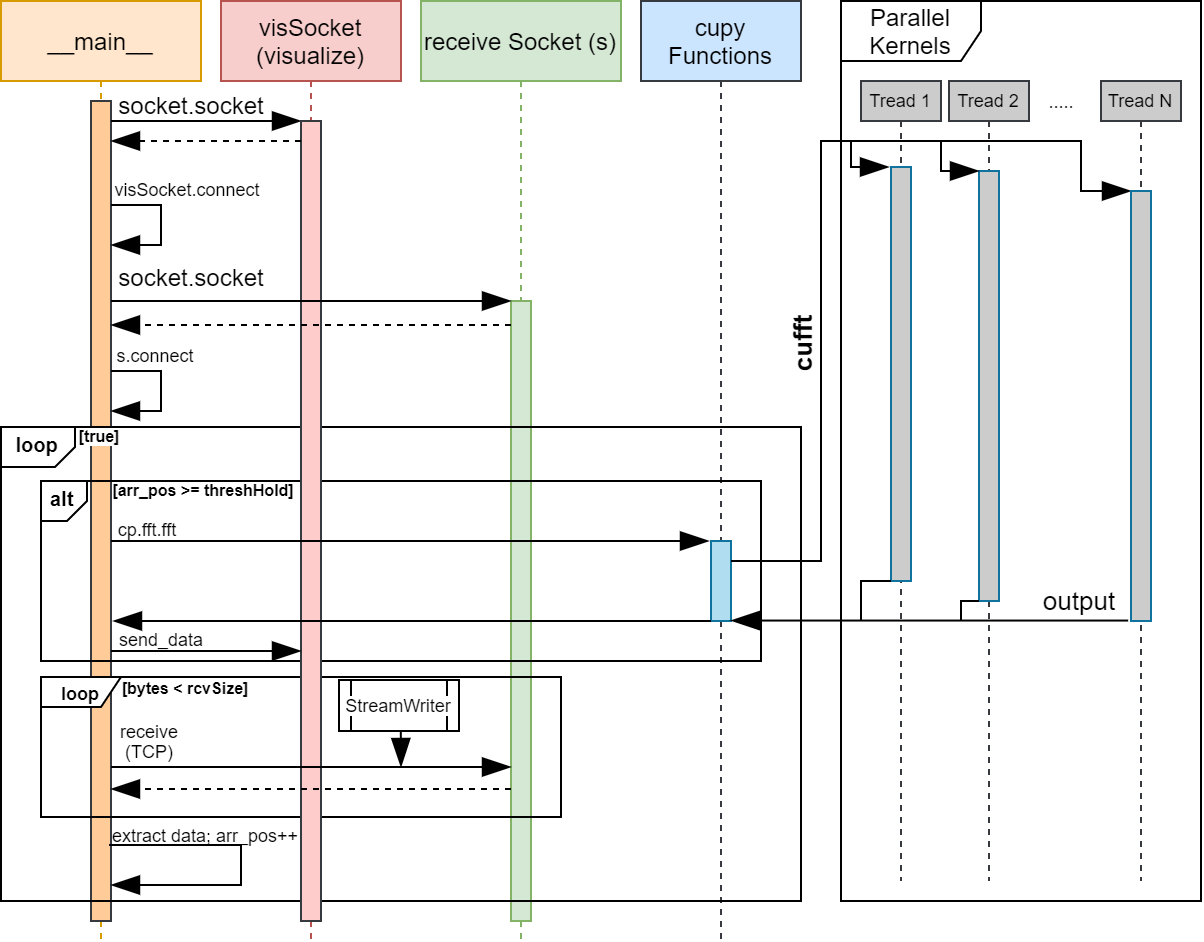
\includegraphics[scale=0.46, angle=-90]{figures/AudioTracerPython_sequence_diagram.png}
	\caption{Sequenzdiagramm AudioTracer-Python}
	\label{fig:Seq_AudioTracer_python}
\end{figure}

\subsection{Bokeh Server zur Livevisualisierung}
\label{sec:bokeh}
Das Bokeh Modul besteht aus einem Webserver, der individuelle Datenmengen an den Browser übertragen kann, der diese mithilfe von JavaScript in eine Grafik visualisiert. Bokeh erlaubt die Übertragung von Daten über POST-Requests an eine vorgegebene Daten-URL. Die Erstellung der nötigen Komponenten und Parameter wird in Abbildung \ref{fig:bokehPlot} demonstriert.

\begin{figure}[t!]
	\lstinputlisting[frame=none, language=C, firstline=77, lastline=90, firstnumber=77 ]{../../Master\_parallel\_fourier\_audio/python/visServer.py}
	\caption{Erstellung eines Plots mit Ajax Datenübertragung}
	\label{fig:bokehPlot}
\end{figure}

Die Datenquelle ist durch die Methode AjaxDataSource vorgegeben (Z. 78). Die drei angegebenen Parameter geben folgende Informationen an:

\begin{itemize}
	\item data\_url: Angabe der URL, auf der die Daten empfangen werden
	\item polling\_interval: Angabe des Polling Intervalls der Daten auf gegebener URL in Millisekunden
	\item adapter: Ein individuell erstellter JavaScript Adapter, der angibt wie die empfangenen Daten an die Visualisierung weitergegeben werden. Dazu mehr im Kontext von Abbildung \ref{fig:visAdapter}
\end{itemize}

Es besteht die Möglichkeit, die Datenpunkten mit individuellen Tooltips zu verknüpfen. In Zeilen 81 bis 84 wird ein Tooltip erstellt, der die Eindeutige Nummer, sowie die Lage im Koordinatensystem abgibt.
Die Erstellung des Plots wird mit der Funktion figure vorgenommen (Z.86f.). Hier können unter anderem Größe und Hintergrundfarbe des Plots, sowie der zuvor erstellte Tooltip angegeben werden. Im Anschluss werden Dimensionen der X- und Y-Achse festgelegt. Da die Schallempfindung des menschlichen Ohrs im Durchschnitt zwischen 20Hz und 20kHz stattfindet, liegt die Dimension der X-Achse im Bereich von -25000(Hz) bis 25000(Hz). An dieser Stelle sei anzumerken, dass die Ausgabe einer Fouriertransformation auch negative Werte zulässt, da auch negative Frequenzen zum Ausgangssignal \enquote{passen}. Die Datenpunkte werden als Kreisförmiger Punkt in einem zweidimensionalen Koordinatensystem angegeben. Der Parameter \texttt{source} gibt die zuvor thematisierte Datenquelle an.

\begin{addmargin}[1cm]{1cm}
\textbf{Einschub:}\\
Die Fouriertransformierten Daten geben den Ausschlag einer Frequenz in einem bestimmten Hertz Bereich an. Diese liegen in sogenannten Buckets vor. Diese Buckets sind von der Sample Rate und Größe der Datenmengen abhängig. Das allgemeine Beispiel gibt eine Sample Rate von 44,1kHz und eine Größe von 5000 Samples an. Daraus können Frequenz-Buckets berechnet werden, die in Korrelation zu den berechneten Daten anhand der Position im Ausgabearray stehen.  Dabei enthält die Ausgabe sowohl positive als auch negative Zuordnungen.
\begin{lstlisting}[language=Python, frame=none, numbers=none]
freq_buckets = list()
for i in range(0, int(threshHold/2)):
freq_buckets.append(i * sample_rate / threshHold)

for i in range(int(-threshHold/2), 0):
freq_buckets.append(i * sample_rate / threshHold)
\end{lstlisting}

Die erste Hälfte der Daten enthalten die positiven Frequenzeinträge. Analog werden negative Frequenz-Buckets in der zweiten Hälfte angegeben. Die Berechnung eines Buckets ist definiert durch: $i * sample_rate / size$. Die Variable i beschreibt den fortlaufenden Index eines solchen Buckets und size die Größe der Eingabedaten, was in diesem Kontext mit threshHold gleichzustellen ist. So würde die Berechnung für die Beispielindizes 100 und 101 die Frequenzen 882 bzw. 890,2 ergeben. Hier wird ein sehr wichtiger Punkt klar: Die Größe einer Fouriertransformation bestimmt zugleich deren Genauigkeit. Mit dem oben angegebenen Beispiel kann Der Frequenznbereich zwischen 882 und 890,2 bei einer Größe von 5000 Eingabesamples niemals abgebildet werden.
\end{addmargin}

Die Frequenz-Buckets werden im Plot Koordinatensystem in X-Richtung angegeben. Auf der Y-Achse stehen die errechneten Ausschläge für die entsprechenden Frequenzen. 
Die Übertragung in das Plot-Koordinatensystem erfolgt mit dem zuvor erwähnten JavaScript Adapter aus Abbildung \ref{fig:bokehPlot}. 

\begin{figure}[t!]
	\lstinputlisting[frame=none, language=Python, firstline=58, lastline=75, firstnumber=58 ]{../../Master\_parallel\_fourier\_audio/python/visServer.py}
	\caption{Erstellung eines Plots mit Ajax Datenübertragung}
	\label{fig:bokehPlot}
\end{figure}

Der JavaScript Code des Adapters wird in Form eines String erstellt, der dem Browser zum Zeitpunkt der Verbindung übermittelt wird. Dieser wird ausgeführt, sobald Daten über die URL \texttt{http://localhost:{port}/data} empfangen wurde. Die Empfangenen Daten werden in Koordinatenpunkte des Plots umgewandelt und der Visualisierung angefügt.
Der Python Webserver übermittelt in Form von JSON-Strings. Auf die Browser-Anfrage auf  o.g. URL reagiert die folgende Implementierung:

\begin{lstlisting}[language=Python, frame=none, numbers=none]
@app.route('/data', methods=['GET', 'OPTIONS', 'POST'])
@crossdomain
def data():
return json.dumps({'frequency_buckets': freq_buckets, 'magnitudes': list(magnitudeHolder),
	'channels': channels, 'size': threshHold})
\end{lstlisting}

Die Annotation \texttt{@app.route} gewährleistet, dass die definierte Funktion auf Anfragen der URL /data ausgeführt wird. Eine weitere Annotation \texttt{@crossdomain} liefert die hierfür nötigen Response-Header. Der Server schickt dem Browser Informationen über die Frequenz-Buckets, die dazu berechneten Fouriertransformierten Daten (aufgeteilt auf die Kanäle), sowie die wichtigen Angaben für Anzahl der Kanäle und Größe der Samples.

Abhängig vom angegebenen Polling Intervall werden so die Daten ständig an den Browser übertragen. Das Python Modul kann von beiden AudioTracer Modulen Daten empfangen und verarbeiten. Das gleichzeitige Empfangen von beiden Endpunkten ist dabei nicht möglich.

\begin{figure}[hbt!]
	\centering      
	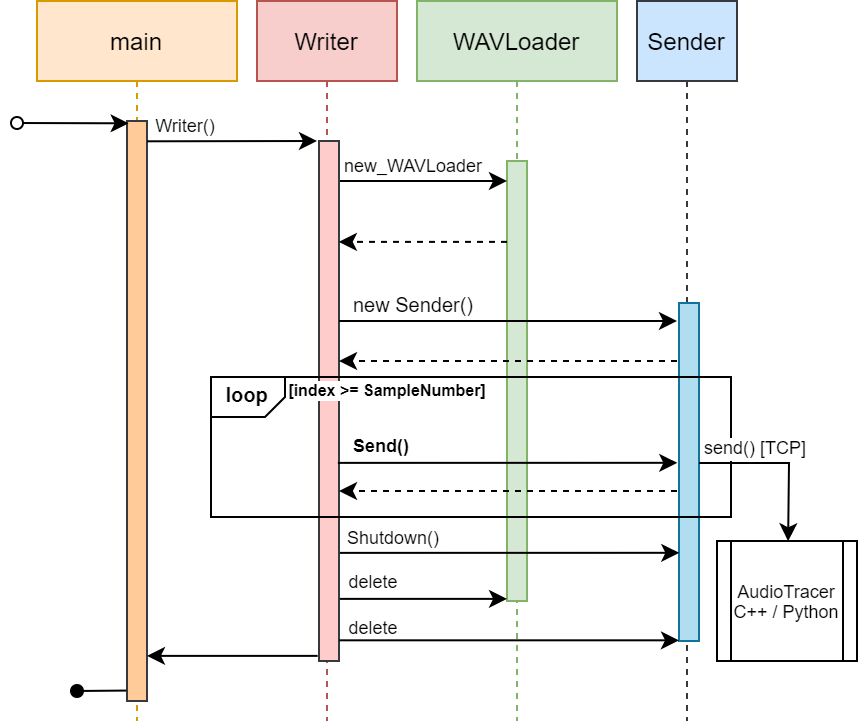
\includegraphics[scale=0.5]{figures/StreamWriter_sequence_diagram.png}
	\caption{Sequenzdiagramm StreamWriter}
	\label{fig:Seq_StreamWriter}
\end{figure}


